\documentclass[11pt, reqno]{article}   	% use "amsart" instead of "article" for AMSLaTeX format
\usepackage{my_packages}

\title{Dynamics near asteroids}
\author{Shankar Kulumani}
\date{18 Feb 2016}							% Activate to display a given date or no date

\begin{document}
\maketitle

\subsection*{Dynamics}

I am beginning by modeling the asteroid as a rotating, constant density triaxial ellipsoid. 
The gravitational potential can be simplified to a second degree and order model and captures the major perturbations due to the non-spherical shape of the body.
A body fixed frame is centered at the center of mass of the asteroid and aligned with the principle axes. 
We also assume \( I_{xx} \leq I_{yy} \leq I_{zz} \) and the semi-axes \( \gamma \leq \beta \leq \alpha \).
The second order and degree potential coefficients are related to the moments of inertia by 
\begin{align*}
	C_{20} &= -\frac{1}{2} M \parenth{2 I_{zz} - I_{xx} - I_{yy}} , \\
	C_{22} &=  \frac{1}{4} \parenth{I_{yy} - I_{xx}} .
\end{align*}
The gravitational potential is given by
\begin{align*}
	U = \frac{\mu}{r} + \frac{\mu}{r^3} \bracket{C_{20} \parenth{1-\frac{3}{2} \cos^2 \delta} + \frac{3 C_{22} \parenth{x^2 - y^2}}{r^5} } ,
\end{align*}
where \( \vecbf{r} = \begin{bmatrix} x & y & z \end{bmatrix}^T \) and \( \mu = G M \) is the gravitational parameter of the asteroid.
In a rotating reference frame fixed to the asteroid the equations of motion of a massless particle are given by
\begin{align*}
	\ddot{x} - 2 \omega \dot{y} &= \omega^2 x - \frac{\mu x}{r^3} + \deriv{U_2}{x} \\
	\ddot{y} + 2 \omega \dot{x} &= \omega^2 y - \frac{\mu y}{r^3} + \deriv{U_2}{y} \\
	\ddot{z} &= -\frac{\mu z}{r^3} + \deriv{U_2}{z} 
\end{align*}
with the partial derivatives of the non-spherical potential components given by
\begin{align*}
	\deriv{U_2}{x} &= -\frac{\mu}{r^5} C_{20} x + \frac{5 \mu C_{20} x \parenth{x^2 + y^2 - 2 z^2}}{2 r^7} + \frac{6 \mu C_{22}x}{r^5} - \frac{15 \mu C_{22} x \parenth{x^2 - y^2}}{r^7} , \\
	\deriv{U_2}{y} &= -\frac{\mu C_{20} y}{r^5} + \frac{5 \mu C_{20} y \parenth{x^2+y^2-2z^2}}{2 r^7} - \frac{6 \mu C_{22}y}{r^5} - \frac{15 \mu C_{22} y \parenth{x^2 - y^2}}{r^7}, \\
	\deriv{U_2}{z} &= \frac{2 \mu C_{20} z}{r^5} + \frac{5 \mu C_{20} z \parenth{x^2 + y^2 - 2 z^2}}{2 r^7} - \frac{15 \mu C_{22} z \parenth{x^2-y^2}}{r^7}.
\end{align*}
Since the gravitational potential is time invariant we can define a constant of integration as
\begin{align*}
	J = \frac{1}{2} \parenth{\dot{x}^ + \dot{y}^2 + \dot{z}^2} - \frac{1}{2} \omega^2 \parenth{x^2 + y^2} - U_2 - \frac{\mu}{r} .
\end{align*}
I believe this also means that any other gravitational potential model could also be used as the only requirement is time invariance.

\subsubsection*{Nondimensionalization}
In order to nondimensionalize the system we define a distance and time scale factor
\begin{align*}
	r_s = \parenth{\frac{\mu}{\omega^2}}^{\frac{1}{3}} \quad \tau = \omega t .	
\end{align*}
Using these the state is redefined as
\begin{align*}
	\tilde{x} &= \frac{x}{r_2} \quad \tilde{y} = \frac{y}{r_s} \quad \tilde{z} = \frac{z}{r_s}, \\
	\dot{\tilde{x}} &= \frac{\dot{x}}{\omega r_2} \quad \dot{\tilde{y}} = \frac{\dot{y}}{\omega r_s} \quad \dot{\tilde{z}} = \frac{\dot{z}}{r_s},\\
	\ddot{\tilde{x}} &= \frac{\ddot{x}}{\omega^2 r_2} \quad \ddot{\tilde{y}} = \frac{\ddot{y}}{\omega^2 r_s} \quad \ddot{\tilde{z}} = \frac{\ddot{z}}{\omega^2 r_s} .
\end{align*}
And the potential parameters become \( \tilde{C_{20}} = \frac{C_{20}}{r_s^2}, \tilde{C_{22}} = \frac{C_{22}}{r_s^2} \).
Using these new relations and dropping the tilde notation the nondimensional equations of motion are given by
\begin{align*}
	\ddot{x} - 2 \dot{y} &= x - \frac{x}{r^3} + \deriv{U_2}{x}, \\
	\ddot{y} + 2 \dot{x} &=  y - \frac{y}{r^3} + \deriv{U_2}{y}, \\
	\ddot{z} &= -\frac{z}{r^3} + \deriv{U_2}{z} .
\end{align*}
The second order gravitatational potential in cartesian coordinates becomes
\begin{align*}
	U_s = \frac{C_{20} \parenth{x^2+y^2-2z^2}}{2 r^5} + \frac{3 C_{22} \parenth{x^2 - y^2}}{r^5} .
\end{align*}
The gradient is found by setting \( \mu =1 \) in the above dimensional relations.

Dr. Scheeres used a spherical harmonic expansion up to order 16 and demonstrated periodic orbits and stable/unstable manifolds around 4769 Castalia~\cite{scheeres1996}.
I'm attempting to use his values to see if only a second order potential is able to capture some of the same behavior. 
For example, I created the contour plot in~\cref{fig:2nd_castalia} of the zero velocity curves about 4769 Castalia.
\begin{figure}
	\centering
	\begin{subfigure}[b]{0.5\textwidth}
	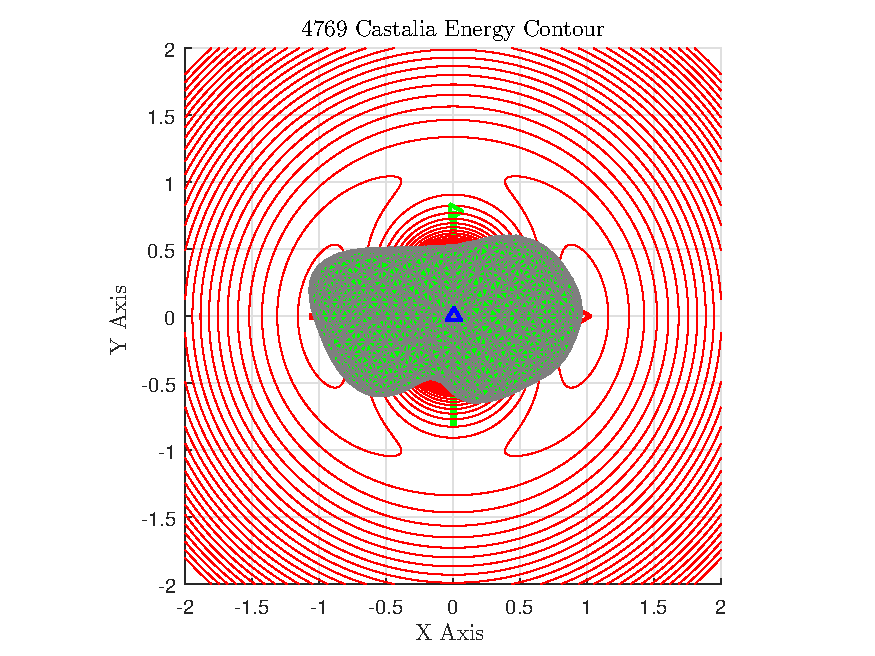
\includegraphics[width=\textwidth]{castalia_zero_velocity_curves}
	\caption{2nd Order ZVC\label{fig:2nd_castalia}}
	\end{subfigure}~
	\begin{subfigure}[b]{0.5\textwidth}
	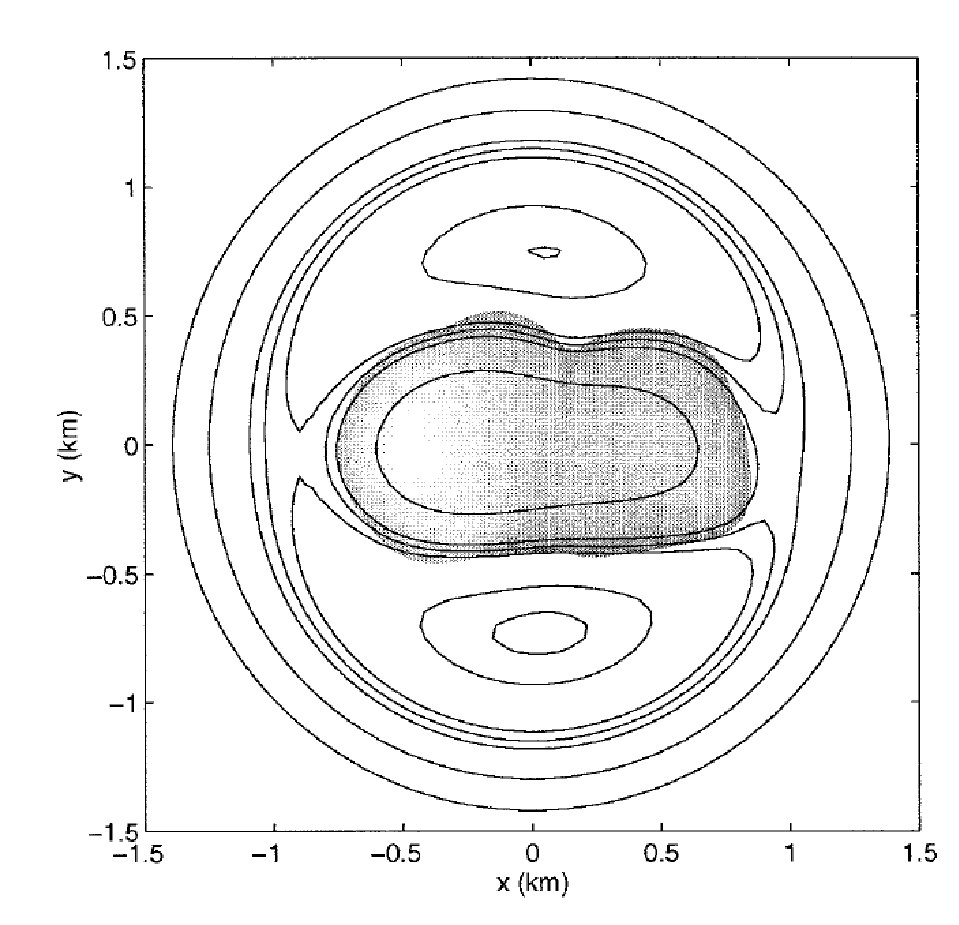
\includegraphics[width=\textwidth]{scheeres_castalia}
	\caption{16th order ZVC\label{fig:castalia}}
	\end{subfigure}
\end{figure}
The zero velocity curves determined using a higher order model is shown in~\cref{fig:castalia}.
Comparing the two shows that the contours from the lower order model seem to be rotated by \SI{90}{\degree}.
This seems to suggest that gravitational model (and it's accuracy) plays a very important role in defining equilibrium points and invaraint manifolds.
One possible source of the difference is that the spherical harmonic model is not accurate when close to surface, where higher order terms are more dominant.

Another issue I've found is trying to find detailed information on the shape/potential for asteroids.
Different researchers use various methods of normalizing the gravity parameters. 
As a result it makes it difficult to compare results between papers or to try and duplicate results.
\bibliographystyle{abbrv}
%\bibliography{../../../../docs/technical_papers/bibtex/library}
\bibliography{library}
\end{document}  